% Inline Autogyro — Tube Capture & Stack Connection
% Compile: pdflatex tube_capture.tex
\documentclass[tikz,border=14pt]{standalone}
\usepackage{tikz}
\usetikzlibrary{arrows.meta,calc,patterns,decorations.pathreplacing,positioning,shapes.geometric}

\begin{document}
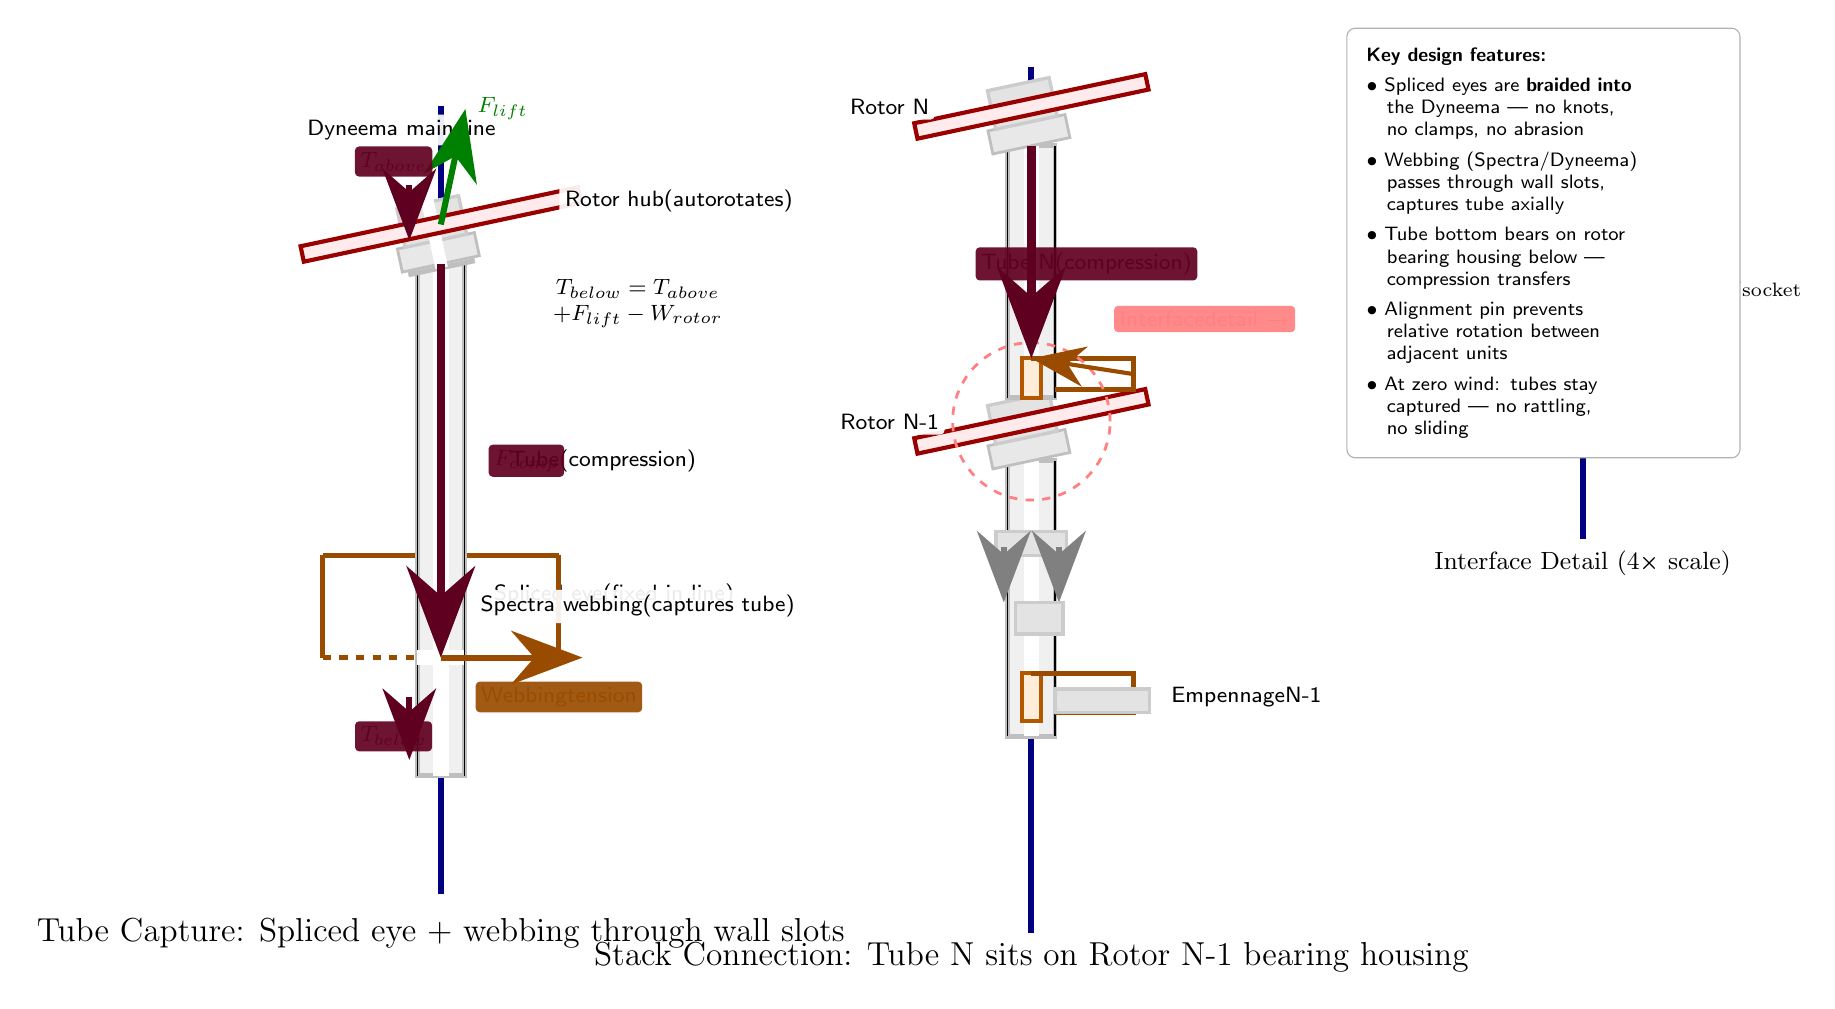
\begin{tikzpicture}[
    scale=1.0,
    dyneema/.style={draw=blue!50!black, line width=2.2pt},
    tube/.style={draw=gray!50, fill=gray!12, line width=1.8pt},
    metal/.style={draw=gray!40, fill=gray!22, line width=1.2pt},
    bearing/.style={draw=gray!50, fill=gray!18, line width=1.0pt},
    splice/.style={draw=orange!70!black, fill=orange!15, line width=1.5pt},
    webbing/.style={draw=orange!60!black, line width=1.8pt},
    rotor/.style={draw=red!60!black, fill=red!8, line width=1.5pt},
    force/.style={-{Stealth[scale=2.0]}, line width=2.2pt},
    annot/.style={font=\footnotesize\sffamily, fill=white, fill opacity=0.92,
                  text opacity=1, inner sep=2pt, rounded corners=1.5pt},
    label/.style={font=\small\sffamily\bfseries},
]

\def\tilt{12}

% =============================================================
% ZOOMED DETAIL: Tube capture mechanism (left half)
% =============================================================

\begin{scope}[local bounding box=detail, shift={(0,0)}]

% Dyneema line
\draw[dyneema] (0, -0.5) -- (0, 9.5);
\node[annot] at (-0.5, 9.2) {Dyneema main line};

% === SPLICED EYE IN DYNEMA ===
% Show the splice as a braided bulge in the line
\fill[splice] (-0.15, 2.8) rectangle (0.15, 3.8);
\draw[splice] (-0.15, 2.8) -- (0.15, 2.8);
\draw[splice] (-0.15, 3.8) -- (0.15, 3.8);
% Eye at top of splice
\draw[webbing] (0, 3.8) circle (0.3);

\node[annot, right=0.3cm] at (0.3, 3.3) {Spliced eye\\(fixed in line)};

% === WEBBING / SPECTRA LOOPS ===
% From the spliced eye, webbing passes through tube wall slots
\draw[webbing] (0, 3.8) -- (1.5, 3.8);
\draw[webbing] (0, 3.8) -- (-1.5, 3.8);
% Down the outside of the tube
\draw[webbing] (1.5, 3.8) -- (1.5, 2.5);
\draw[webbing] (-1.5, 3.8) -- (-1.5, 2.5);
% Through slots in tube wall
\draw[webbing, dashed] (1.5, 2.5) -- (0.3, 2.5);
\draw[webbing, dashed] (-1.5, 2.5) -- (-0.3, 2.5);

\node[annot] at (2.5, 3.15) {Spectra webbing\\(captures tube)};

% === TUBE ===
% Main tube body (shown in cross-section)
\fill[tube] (-0.3, 1.0) rectangle (0.3, 7.5);
% Inner hole for line
\fill[white] (-0.1, 1.0) rectangle (0.1, 7.5);
\draw[thin] (-0.3, 1.0) -- (-0.3, 7.5);
\draw[thin] (0.3, 1.0) -- (0.3, 7.5);
% Wall slots for webbing (at bottom of tube)
\fill[white] (-0.3, 2.4) rectangle (0.3, 2.6);

\node[annot, right=0.4cm] at (0.4, 5.0) {Tube\\(compression)};

% Tube top — angled bearing seat
\begin{scope}
    \clip (-2, 6.8) rectangle (2, 8.0);
    \fill[tube, rotate around={\tilt:(0,7.5)}] (-0.4, 7.45) rectangle (0.4, 7.7);
\end{scope}

% === BEARING & ROTOR (above) ===
\fill[bearing, rotate around={\tilt:(0,7.5)}] (-0.5, 7.5) rectangle (0.5, 7.8);
\fill[metal, rotate around={\tilt:(0,7.5)}] (-0.4, 7.8) rectangle (0.4, 8.3);
\fill[white, rotate around={\tilt:(0,7.5)}] (-0.08, 7.45) rectangle (0.08, 8.4);

% Rotor disk
\fill[rotor, rotate around={\tilt:(0,8.0)}] (-1.8, 7.9) rectangle (1.8, 8.1);

\node[annot, right=0.3cm] at (1.2, 8.3) {Rotor hub\\(autorotates)};

% === FORCE PATH ===
% Lift from rotor
\draw[force, green!50!black] (0, 8.0) -- ++({1.5*sin(\tilt)}, {1.5*cos(\tilt)})
    node[right, font=\footnotesize\sffamily, green!50!black] {$F_\text{lift}$};

% Compression through tube
\draw[force, purple!50!black, line width=3pt] (0, 7.5) -- (0, 2.5);
\node[annot, purple!50!black, right=0.1cm] at (0.5, 5.0) {$F_\text{comp}$};

% Load transfer into webbing
\draw[force, orange!60!black] (0, 2.5) -- (1.8, 2.5);
\node[annot, orange!60!black] at (1.5, 2.0) {Webbing\\tension};

% Tension step in Dyneema
\node[annot, purple!50!black] at (-0.6, 8.8) {$T_\text{above}$};
\node[annot, purple!50!black] at (-0.6, 1.5) {$T_\text{below}$};
\draw[force, purple!50!black] (-0.4, 8.5) -- (-0.4, 7.8);
\draw[force, purple!50!black] (-0.4, 2.0) -- (-0.4, 1.2);

% Force sum annotation
\node[annot, align=center] at (2.5, 7.0) {$T_\text{below} = T_\text{above}$\\$+ F_\text{lift} - W_\text{rotor}$};

% Title
\node[label, font=\large] at (0, -1.0) {Tube Capture: Spliced eye + webbing through wall slots};

\end{scope}

% =============================================================
% STACK CONNECTION: How rotor N sits on rotor N-1 (right)
% =============================================================

\begin{scope}[local bounding box=stack, shift={(7.5,0)}]

% Dyneema line
\draw[dyneema] (0, -1.0) -- (0, 10.0);

% === ROTOR N-1 (lower unit) ===
% Tube N-1
\fill[tube] (-0.3, 1.5) rectangle (0.3, 5.0);
\fill[white] (-0.1, 1.5) rectangle (0.1, 5.0);
\draw[thin] (-0.3, 1.5) -- (-0.3, 5.0);
\draw[thin] (0.3, 1.5) -- (0.3, 5.0);

% Splice N-1
\fill[splice] (-0.12, 1.7) rectangle (0.12, 2.3);
\draw[webbing] (0, 2.3) -- (1.3, 2.3) -- (1.3, 1.8) -- (0.3, 1.8);

% Bearing N-1
\fill[bearing, rotate around={\tilt:(0,5.0)}] (-0.5, 5.0) rectangle (0.5, 5.3);
\fill[metal, rotate around={\tilt:(0,5.0)}] (-0.4, 5.3) rectangle (0.4, 5.8);
\fill[rotor, rotate around={\tilt:(0,5.5)}] (-1.5, 5.4) rectangle (1.5, 5.6);

\node[annot] at (-1.8, 5.5) {Rotor N-1};

% Swashplate + actuators on tube N-1
\fill[metal] (-0.45, 3.8) rectangle (0.45, 4.1);
\draw[force, gray] (-0.35, 3.9) -- (-0.35, 3.2);
\draw[force, gray] (0.35, 3.9) -- (0.35, 3.2);
\fill[metal] (-0.2, 2.8) rectangle (0.4, 3.2);

% Empennage N-1
\fill[metal] (0.3, 1.8) rectangle (1.5, 2.1);

\node[annot, right=0.2cm] at (1.5, 2.0) {Empennage\\N-1};

% === INTERFACE: Tube N-1 top meets Tube N bottom ===
% The bearing housing of rotor N-1 has a flat or cupped top surface
% Tube N sits on this surface

% Tube N
\fill[tube] (-0.3, 5.8) rectangle (0.3, 9.0);
\fill[white] (-0.1, 5.8) rectangle (0.1, 9.0);
\draw[thin] (-0.3, 5.8) -- (-0.3, 9.0);
\draw[thin] (0.3, 5.8) -- (0.3, 9.0);

% Splice N (at bottom of tube N)
\fill[splice] (-0.12, 5.8) rectangle (0.12, 6.3);
\draw[webbing] (0, 6.3) -- (1.3, 6.3) -- (1.3, 5.9) -- (0.3, 5.9);

% Bearing N
\fill[bearing, rotate around={\tilt:(0,9.0)}] (-0.5, 9.0) rectangle (0.5, 9.3);
\fill[metal, rotate around={\tilt:(0,9.0)}] (-0.4, 9.3) rectangle (0.4, 9.8);
\fill[rotor, rotate around={\tilt:(0,9.5)}] (-1.5, 9.4) rectangle (1.5, 9.6);

\node[annot] at (-1.8, 9.5) {Rotor N};

% === INTERFACE DETAIL (zoom circle) ===
\draw[red!50, line width=1pt, dashed] (0, 5.5) circle (1.0);
\node[annot, red!50] at (2.2, 6.8) {Interface\\detail →};

% === FORCE PATH THROUGH STACK ===
% Tube N in compression
\draw[force, purple!50!black, line width=3pt] (0, 9.0) -- (0, 6.3);
% Splice N transfers load into Dyneema
\draw[force, orange!60!black, line width=1.5pt] (1.3, 6.1) -- (0, 6.3);

\node[annot, purple!50!black] at (0.7, 7.5) {Tube N\\(compression)};

% Title
\node[label, font=\large] at (0, -1.3) {Stack Connection: Tube N sits on Rotor N-1 bearing housing};

\end{scope}

% =============================================================
% INTERFACE DETAIL: zoomed callout (bottom right)
% =============================================================

\begin{scope}[local bounding box=iface, shift={(14.5,4.5)}]

% Dyneema
\draw[dyneema] (0, -0.5) -- (0, 4.0);

% Bearing housing of rotor N-1 (lower)
\fill[bearing] (-0.6, 1.5) rectangle (0.6, 2.2);
\fill[metal] (-0.5, 2.2) rectangle (0.5, 2.5);
% Flat top surface
\draw[line width=1pt] (-0.6, 2.5) -- (0.6, 2.5);

% Tube N bottom (sits on bearing housing)
\fill[tube] (-0.35, 2.5) rectangle (0.35, 3.5);
\fill[white] (-0.1, 2.5) rectangle (0.1, 3.5);

% Splice at bottom of tube N
\fill[splice] (-0.12, 2.5) rectangle (0.12, 2.9);
\draw[webbing] (0, 2.9) -- (1.0, 2.9) -- (1.0, 2.6) -- (0.35, 2.6);

% Optional: alignment pin/socket
\fill[metal] (0.5, 2.5) rectangle (0.65, 2.8);
\fill[white] (0.5, 2.5) rectangle (0.68, 2.55);
\draw[thin] (0.45, 2.5) -- (0.7, 2.5);

\node[annot, font=\scriptsize] at (1.5, 2.65) {Alignment\\pin/socket};

% Load arrows
\draw[force, purple!50!black, line width=2pt] (0, 3.5) -- (0, 2.5)
    node[midway, right, annot, purple!50!black] {Compression};
\draw[force, orange!60!black, line width=1.5pt] (0, 2.9) -- (1.3, 2.9)
    node[midway, above, font=\tiny\sffamily, orange!60!black] {Webbing tension};

% Title
\node[label, font=\small] at (0, -0.8) {Interface Detail (4× scale)};

\end{scope}

% === ANNOTATIONS (design notes) ===
\node[draw=black!30, fill=white, rounded corners=3pt, inner sep=7pt,
      anchor=north west, font=\scriptsize\sffamily, align=left, text width=4.5cm]
    at (11.5, 10.5) {
    \textbf{Key design features:}\\[3pt]
    $\bullet$ Spliced eyes are \textbf{braided into}\\\quad the Dyneema — no knots,\\\quad no clamps, no abrasion\\[3pt]
    $\bullet$ Webbing (Spectra/Dyneema)\\\quad passes through wall slots,\\\quad captures tube axially\\[3pt]
    $\bullet$ Tube bottom bears on rotor\\\quad bearing housing below —\\\quad compression transfers\\[3pt]
    $\bullet$ Alignment pin prevents\\\quad relative rotation between\\\quad adjacent units\\[3pt]
    $\bullet$ At zero wind: tubes stay\\\quad captured — no rattling,\\\quad no sliding
};

\end{tikzpicture}
\end{document}
